% Auto-generated by the analysis pipeline — do not edit
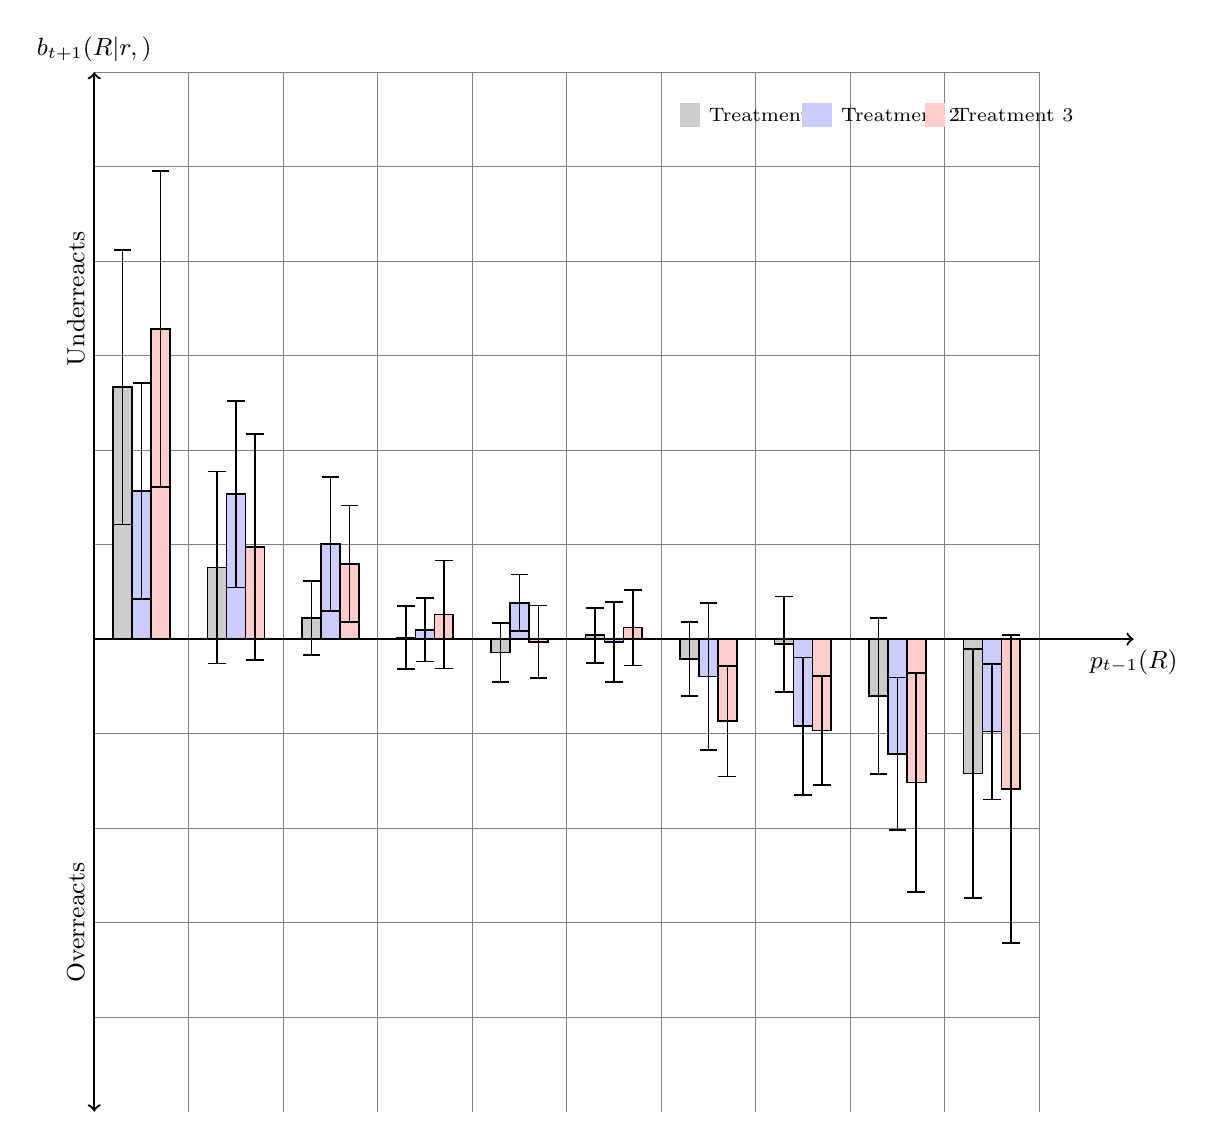
\begin{tikzpicture}[scale=12]
\draw[help lines,step=0.1] (0,-0.5) grid (1,0.6);
\filldraw[opaque,white!80!black] (0.0200,0) rectangle (0.0400,0.2667);
\draw[line width=0.6] (0.0200,0) rectangle (0.0400,0.2667);
\draw[line width=0.6,|-|] (0.0300,0.1204) -- (0.0300,0.4129);
\filldraw[opaque,white!80!blue] (0.0400,0) rectangle (0.0600,0.1568);
\draw[line width=0.6] (0.0400,0) rectangle (0.0600,0.1568);
\draw[line width=0.6,|-|] (0.0500,0.0414) -- (0.0500,0.2722);
\filldraw[opaque,white!80!red] (0.0600,0) rectangle (0.0800,0.3281);
\draw[line width=0.6] (0.0600,0) rectangle (0.0800,0.3281);
\draw[line width=0.6,|-|] (0.0700,0.1598) -- (0.0700,0.4964);
\filldraw[opaque,white!80!black] (0.1200,0) rectangle (0.1400,0.0757);
\draw[line width=0.6] (0.1200,0) rectangle (0.1400,0.0757);
\draw[line width=0.6,|-|] (0.1300,-0.0267) -- (0.1300,0.1781);
\filldraw[opaque,white!80!blue] (0.1400,0) rectangle (0.1600,0.1533);
\draw[line width=0.6] (0.1400,0) rectangle (0.1600,0.1533);
\draw[line width=0.6,|-|] (0.1500,0.0538) -- (0.1500,0.2528);
\filldraw[opaque,white!80!red] (0.1600,0) rectangle (0.1800,0.0973);
\draw[line width=0.6] (0.1600,0) rectangle (0.1800,0.0973);
\draw[line width=0.6,|-|] (0.1700,-0.0232) -- (0.1700,0.2179);
\filldraw[opaque,white!80!black] (0.2200,0) rectangle (0.2400,0.0224);
\draw[line width=0.6] (0.2200,0) rectangle (0.2400,0.0224);
\draw[line width=0.6,|-|] (0.2300,-0.0174) -- (0.2300,0.0621);
\filldraw[opaque,white!80!blue] (0.2400,0) rectangle (0.2600,0.1009);
\draw[line width=0.6] (0.2400,0) rectangle (0.2600,0.1009);
\draw[line width=0.6,|-|] (0.2500,0.0290) -- (0.2500,0.1727);
\filldraw[opaque,white!80!red] (0.2600,0) rectangle (0.2800,0.0797);
\draw[line width=0.6] (0.2600,0) rectangle (0.2800,0.0797);
\draw[line width=0.6,|-|] (0.2700,0.0171) -- (0.2700,0.1423);
\filldraw[opaque,white!80!black] (0.3200,0) rectangle (0.3400,0.0016);
\draw[line width=0.6] (0.3200,0) rectangle (0.3400,0.0016);
\draw[line width=0.6,|-|] (0.3300,-0.0326) -- (0.3300,0.0359);
\filldraw[opaque,white!80!blue] (0.3400,0) rectangle (0.3600,0.0097);
\draw[line width=0.6] (0.3400,0) rectangle (0.3600,0.0097);
\draw[line width=0.6,|-|] (0.3500,-0.0247) -- (0.3500,0.0440);
\filldraw[opaque,white!80!red] (0.3600,0) rectangle (0.3800,0.0260);
\draw[line width=0.6] (0.3600,0) rectangle (0.3800,0.0260);
\draw[line width=0.6,|-|] (0.3700,-0.0321) -- (0.3700,0.0840);
\filldraw[opaque,white!80!black] (0.4200,0) rectangle (0.4400,-0.0142);
\draw[line width=0.6] (0.4200,0) rectangle (0.4400,-0.0142);
\draw[line width=0.6,|-|] (0.4300,-0.0461) -- (0.4300,0.0178);
\filldraw[opaque,white!80!blue] (0.4400,0) rectangle (0.4600,0.0382);
\draw[line width=0.6] (0.4400,0) rectangle (0.4600,0.0382);
\draw[line width=0.6,|-|] (0.4500,0.0074) -- (0.4500,0.0691);
\filldraw[opaque,white!80!red] (0.4600,0) rectangle (0.4800,-0.0029);
\draw[line width=0.6] (0.4600,0) rectangle (0.4800,-0.0029);
\draw[line width=0.6,|-|] (0.4700,-0.0422) -- (0.4700,0.0364);
\filldraw[opaque,white!80!black] (0.5200,0) rectangle (0.5400,0.0041);
\draw[line width=0.6] (0.5200,0) rectangle (0.5400,0.0041);
\draw[line width=0.6,|-|] (0.5300,-0.0260) -- (0.5300,0.0341);
\filldraw[opaque,white!80!blue] (0.5400,0) rectangle (0.5600,-0.0031);
\draw[line width=0.6] (0.5400,0) rectangle (0.5600,-0.0031);
\draw[line width=0.6,|-|] (0.5500,-0.0464) -- (0.5500,0.0401);
\filldraw[opaque,white!80!red] (0.5600,0) rectangle (0.5800,0.0121);
\draw[line width=0.6] (0.5600,0) rectangle (0.5800,0.0121);
\draw[line width=0.6,|-|] (0.5700,-0.0289) -- (0.5700,0.0531);
\filldraw[opaque,white!80!black] (0.6200,0) rectangle (0.6400,-0.0211);
\draw[line width=0.6] (0.6200,0) rectangle (0.6400,-0.0211);
\draw[line width=0.6,|-|] (0.6300,-0.0611) -- (0.6300,0.0190);
\filldraw[opaque,white!80!blue] (0.6400,0) rectangle (0.6600,-0.0396);
\draw[line width=0.6] (0.6400,0) rectangle (0.6600,-0.0396);
\draw[line width=0.6,|-|] (0.6500,-0.1185) -- (0.6500,0.0394);
\filldraw[opaque,white!80!red] (0.6600,0) rectangle (0.6800,-0.0870);
\draw[line width=0.6] (0.6600,0) rectangle (0.6800,-0.0870);
\draw[line width=0.6,|-|] (0.6700,-0.1465) -- (0.6700,-0.0276);
\filldraw[opaque,white!80!black] (0.7200,0) rectangle (0.7400,-0.0055);
\draw[line width=0.6] (0.7200,0) rectangle (0.7400,-0.0055);
\draw[line width=0.6,|-|] (0.7300,-0.0569) -- (0.7300,0.0459);
\filldraw[opaque,white!80!blue] (0.7400,0) rectangle (0.7600,-0.0923);
\draw[line width=0.6] (0.7400,0) rectangle (0.7600,-0.0923);
\draw[line width=0.6,|-|] (0.7500,-0.1658) -- (0.7500,-0.0188);
\filldraw[opaque,white!80!red] (0.7600,0) rectangle (0.7800,-0.0969);
\draw[line width=0.6] (0.7600,0) rectangle (0.7800,-0.0969);
\draw[line width=0.6,|-|] (0.7700,-0.1552) -- (0.7700,-0.0385);
\filldraw[opaque,white!80!black] (0.8200,0) rectangle (0.8400,-0.0600);
\draw[line width=0.6] (0.8200,0) rectangle (0.8400,-0.0600);
\draw[line width=0.6,|-|] (0.8300,-0.1435) -- (0.8300,0.0235);
\filldraw[opaque,white!80!blue] (0.8400,0) rectangle (0.8600,-0.1214);
\draw[line width=0.6] (0.8400,0) rectangle (0.8600,-0.1214);
\draw[line width=0.6,|-|] (0.8500,-0.2029) -- (0.8500,-0.0399);
\filldraw[opaque,white!80!red] (0.8600,0) rectangle (0.8800,-0.1517);
\draw[line width=0.6] (0.8600,0) rectangle (0.8800,-0.1517);
\draw[line width=0.6,|-|] (0.8700,-0.2687) -- (0.8700,-0.0347);
\filldraw[opaque,white!80!black] (0.9200,0) rectangle (0.9400,-0.1424);
\draw[line width=0.6] (0.9200,0) rectangle (0.9400,-0.1424);
\draw[line width=0.6,|-|] (0.9300,-0.2750) -- (0.9300,-0.0097);
\filldraw[opaque,white!80!blue] (0.9400,0) rectangle (0.9600,-0.0979);
\draw[line width=0.6] (0.9400,0) rectangle (0.9600,-0.0979);
\draw[line width=0.6,|-|] (0.9500,-0.1705) -- (0.9500,-0.0253);
\filldraw[opaque,white!80!red] (0.9600,0) rectangle (0.9800,-0.1585);
\draw[line width=0.6] (0.9600,0) rectangle (0.9800,-0.1585);
\draw[line width=0.6,|-|] (0.9700,-0.3222) -- (0.9700,0.0053);
\draw[line width=0.8,->]  (0,0) -- (1.1,0) node[below] {\small{$p_{t-1}(R)$}};
\draw[line width=0.8,<->] (0,-0.5) -- (0,0.6) node[above] {\small{$b_{t+1}(R|r,\xmark)$}};
\draw (0,0.36) node[above,rotate=90] {\small{Underreacts}};
\draw (0,-0.30) node[above,rotate=90] {\small{Overreacts}};
\filldraw[white!80!black] (0.62,0.5420) rectangle (0.64,0.5670);
\node[right] at (0.64,0.5550) {\scriptsize{Treatment 1}};
\filldraw[white!80!blue] (0.75,0.5420) rectangle (0.78,0.5670);
\node[right] at (0.78,0.5550) {\scriptsize{Treatment 2}};
\filldraw[white!80!red] (0.88,0.5420) rectangle (0.90,0.5670);
\node[right] at (0.90,0.5550) {\scriptsize{Treatment 3}};
\end{tikzpicture}
